\section{Experiments} \label{sec:experiments}


\begin{table*}[t]
% \setlength\tabcolsep{3pt}  %可以控制列间距
% \renewcommand{\arraystretch}{1.1} %可以控制行间距
% \footnotesize
\centering
\fontsize{9}{11}\selectfont
\setlength{\tabcolsep}{2.6mm}{
\begin{tabular}{c|l|cccccc}
\toprule
\multicolumn{1}{c|}{\multirow{2}{*} {Type}} & \multicolumn{1}{l|}{\multirow{2}{*} {Model}}   & \multicolumn{3}{c}{WebQSP}   & \multicolumn{3}{c}{CWQ} \\
\cline{3-8}
 \multicolumn{1}{c|}{} & \multicolumn{1}{c|}{}   &F1&Hits@1& Acc &F1&Hits@1& Acc\\ 
\hline
\hline
\multicolumn{1}{c|}{\multirow{4}{*} {EM-based}} & KV-Mem {\scriptsize \cite{miller2016key}} & 34.5 & 46.7 & - & 15.7 & 18.4 & - \\
\multicolumn{1}{c|}{}& NSM$_{+h}$ {\scriptsize \cite{NSM}} &67.4 & 74.3& - & 44.0& 48.8&-   \\
\multicolumn{1}{c|}{}& TransferNet {\scriptsize \cite{shi2021transfernet}} &-  & 71.4 &- &- &48.6 &  - \\
\multicolumn{1}{c|}{}& KGT5 {\scriptsize \cite{KGT5}} &-  &56.1 &- &- & 36.5&  - \\
\hline
\multicolumn{1}{c|}{\multirow{5}{*} {IR-based}} &  GraftNet {\scriptsize \cite{sun-etal-2018-open}} & 60.4 & 66.4 & - & 32.7 & 36.8 & - \\
\multicolumn{1}{c|}{}& PullNet {\scriptsize \cite{sun-etal-2019-pullnet}} & - & 68.1 & - & - &45.9 & - \\
\multicolumn{1}{c|}{}& SR+NSM {\scriptsize \cite{zhang2022subgraph}} &  64.1 & 68.9 &- &47.1& 50.2&- \\
\multicolumn{1}{c|}{}& SR+NSM+E2E {\scriptsize \cite{zhang2022subgraph}} & 64.1  &69.5 &- &46.3&49.3 &-\\
\multicolumn{1}{c|}{}& UniKGQA {\scriptsize \cite{unikgqa}} & 71.0 &77.0& - &49.4& 50.9 &-\\
\hline
\multicolumn{1}{c|}{\multirow{6}{*} {SP-based}}& CBR-KBQA {\scriptsize \cite{CBR-KBQA}} & 72.8 &- &69.9 &70.0 &-& 67.1 \\
\multicolumn{1}{c|}{}& GMT-KBQA {\scriptsize \cite{GMT-KBQA}} & 76.6 &- &73.1 &77.0 &-& 72.2 \\
\multicolumn{1}{c|}{}& UnifiedSKG {\scriptsize \cite{xie-etal-2022-unifiedskg}} & 73.9 &-& -& 68.8& - &-\\
\multicolumn{1}{c|}{}& RnG-KBQA {\scriptsize \cite{rng-kbqa}} & 75.6&-&-&-&-&-\\
\multicolumn{1}{c|}{}& DecAF {\scriptsize \cite{decaf}} & 78.8&82.1&-&-&70.4&-\\
\multicolumn{1}{c|}{}& FC-KBQA {\scriptsize \cite{fc-kbqa}} & 76.9& - &- &56.4& -& -\\
\hline
\multicolumn{1}{c|}{\multirow{8}{*} {LLM-based}} & KD-CoT {\scriptsize \cite{wang2023knowledge}} & 52.5 & 68.6 & - &-  &55.7 & - \\
\multicolumn{1}{c|}{}& Pangu {\scriptsize \cite{pangu}} & 79.6 & - & - & - & - & - \\
\multicolumn{1}{c|}{}& StructGPT {\scriptsize \cite{structgpt}} & - & 72.6 & -  & -  & - & - \\
\multicolumn{1}{c|}{}& ChatKBQA {\scriptsize \cite{chatkbqa}} & 79.8 &83.2& 73.8 &77.8 &82.7 &73.3\\
\multicolumn{1}{c|}{}& ToG-R (GPT-4) {\scriptsize \cite{TOG}} & - & 82.6 & -  & -  & 69.5 & - \\
\multicolumn{1}{c|}{}& G-Retriever {\scriptsize \cite{G-retriever}} & -& 70.1& -& -& -& -\\
\multicolumn{1}{c|}{}& GNN-RAG {\scriptsize \cite{mavromatis2024gnn}} & 73.5 &82.8& -  &60.4& 62.8& - \\
\rowcolor{gray!10}  \multicolumn{1}{c|}{}& \model (Ours) & \textbf{81.2}\scriptsize{$\pm$0.15} & \textbf{84.3}\scriptsize{$\pm$0.16}  & \textbf{75.2}\scriptsize{$\pm$0.10} & \textbf{78.5}\scriptsize{$\pm$0.11} & \textbf{83.1}\scriptsize{$\pm$0.09} & \textbf{74.5}\scriptsize{$\pm$0.07} \\
\bottomrule
\end{tabular}}
\caption{Performance comparison of different types of KGQA methods on WebQSP and CWQ datasets. We present the Mean scores and standard deviations (mean ± std) of five experiments with different random seeds. The best result is highlighted in \textbf{bold}, and the baseline results are taken from corresponding papers.}
\label{tab:main result}
\end{table*}



\subsection{Experiment Settings}

\textbf{Datasets. }
Our experiments were conducted using two well-known datasets: WebQuestionsSP (WebQSP) \cite{webqsp} and ComplexWebQuestions (CWQ) \cite{CWQ}. The dataset statistics are presented in the Appendix. 
Both datasets contain SPARQL queries that correspond to the questions and can be executed on Freebase to obtain answers.

\noindent\textbf{Baselines.}
In this study, we evaluate performance with 22 baselines, which are categorized into four groups: embedding-based (EM-based), information retrieval-based (IR-based), semantic parsing-based (SP-based), and LLM-based methods. For more detailed descriptions of the baselines, please refer to the Appendix.
It is important to note that some methods, such as DecAF~\cite{decaf}, can be classified as multiple groups, specifically IR-based and SP-based. To ensure fairness, we do not include the results of using the oracle entity linking annotations setting, such as RoG \cite{RoG}. We put the performance comparison of the oracle setting in the Appendix.





\noindent\textbf{Evaluation Metrics.}
We use Hits@1, F1, and Acc as primary evaluation metrics following \cite{chatkbqa}. Hits@1 assesses the accuracy of top-1 predicted answer, F1 considers the coverage of all possible answers, and Acc measures the strict exact-match accuracy.
We further assess the quality of generated S-expressions by employing two metrics: the extract match ratio (EM) and the match after beam search ratio (BM) with ground-truth S-expressions, for analytical experiments.

\noindent\textbf{Implementation Details.}
% We employ LLaMA2-7B and LLaMA2-13B \cite{touvron2023llama} as LLM backbones, and then fine-tune LLMs using LoRA \cite{hu2022lora} on WebQSP and CWQ. 
Following ~\citet{chatkbqa}, we fine-tune LLaMA2-7B on WebQSP and LLaMA2-13B on CWQ using LoRA.
We evaluate the impact of backbones and fine-tuning methods in our subsequent experiments. During inference, we utilize beam search to generate multiple logical forms. We select the executable logical form with the highest score to obtain answers. All experiments were done on NVIDIA A6000 GPUs. We only searched the number of retrievals $k$ with values of \{4,8,16,32,64,100\}. 

\subsection{Main Results}
% In this section, we compare our method with all baselines.
As observed from Table \ref{tab:main result}, \model outperforms all baselines across all metrics on both datasets. Notably, on WebQSP dataset, accuracy has improved by 1.6\% compared to the second-best baseline, ChatKBQA, marking new state-of-the-art performance.
Specifically, \model surpasses subgraph retrieval techniques such as SR+NSM and DecAF with 26\% and 2.4\% F1 improvements on WebQSP, respectively, as well as entity and relation retrieval methods like GMT-KBQA with 5.3\% F1 improvement on WebQSP.
This can be attributed to our proposed self-alignment mechanism, which effectively aligns multi-aspect knowledge.
On the other hand, \model also outperforms other LLM-based approaches, such as G-Retriever and ChatKBQA, suggesting that our approach of learning prompt embeddings for retrieval can more flexibly leverage the capabilities of LLMs to utilize retrieval knowledge.


\begin{table}[t]
\setlength\tabcolsep{2pt}  %可以控制列间距
% \renewcommand{\arraystretch}{1.1} %可以控制行间距
\footnotesize
\centering
\fontsize{9}{11}\selectfont
\setlength{\tabcolsep}{3mm}
\begin{tabular}{l|ccccc}
\toprule
 \multicolumn{1}{l|}{\multirow{2}{*} {Model}} & \multicolumn{5}{c}{WebQSP} \\
\cline{2-6}
 \multicolumn{1}{c|}{} &F1&Hits@1& Acc & EM & BM  \\ 
\hline
\hline
\rowcolor{gray!10} \model & \textbf{81.2} & \textbf{84.3} & \textbf{75.2} & \textbf{63.9} & 76.4\\
w/o \textit{SN} & 80.1 & 83.3 & 74.3& 63.6 & \textbf{77.0}\\
w/o \textit{SA} & 79.5 & 82.6 & 73.8 & 63.0 &75.7 \\
w/o \textit{RG} &79.4 & 82.2 &74.3 & 63.4 & 76.7\\
w/o \textit{SA\&RG} & 78.7& 81.0 & 72.5  & 62.1 & 73.6 \\
w/o \textit{SA\&SN}	&79.1	&82.0	&73.8&	63.1&	76.2\\
w/o \textit{ALL} & 76.2 & 79.5 & 70.1 & 59.7 & 72.4  \\
\bottomrule
\end{tabular}
 \caption{Ablation study of sub-modules on WebQSP dataset.}
\label{tab:ablation}
\end{table}



\subsection{Ablation Study}
In this section, we conduct a series of ablation studies to address the following question: 

\textbf{How do the proposed modules improve performance?} Specifically, we conduct experiments against five variants:
1) w/o \textit{SN}: without siamese network, and relevance score is calculated by vector inner product; 2) w/o \textit{SA}: without self-alignment module; 3)  w/o \textit{RG}: without relevance gating module; 4) w/o \textit{SA\&RG}: without both self-alignment and relevance gating modules, where \model obtains prompt embeddings with only MLP. 5) w/o \textit{ALL}: directly appending the retrieval knowledge as context instead of converting retrieval knowledge to prompt embeddings.
As shown in Table \ref{tab:ablation}, we observe that the performance on most metrics decreases when either \textit{SN}, \textit{SA}, or \textit{RG} is removed. This validates the effectiveness of the proposed sub-modules. Furthermore, we find that performance significantly drops when the entire framework is removed, indicating that appending retrieved knowledge directly as context text introduces a large amount of noise, preventing LLMs from focusing on learning the mapping from question to logical form.
Additionally, we notice that the BM is higher in \model w/o \textit{SN} than in \model. This suggests that the ground-truth logical forms are mostly ranked within the top 2 or lower positions during beam search generation, leading to a lower EM.


\begin{table}[t]
% \setlength\tabcolsep{3pt}  %可以控制列间距
\renewcommand{\arraystretch}{1.1} %可以控制行间距
\footnotesize
\centering
\fontsize{9}{11}\selectfont
\setlength{\tabcolsep}{2.8mm}
\begin{tabular}{l|ccccc}
\toprule
 \multicolumn{1}{l|}{\multirow{2}{*} {Model}} & \multicolumn{5}{c}{WebQSP} \\
\cline{2-6}
 \multicolumn{1}{c|}{} &F1&Hits@1& Acc & EM & BM  \\ 
\hline
\hline
\rowcolor{gray!10} \model & \textbf{81.2} & \textbf{84.3} & \textbf{75.2} & \textbf{63.9} & \textbf{76.4} \\
w/o \textit{Relation} & 78.6 & 81.7 &73.1 & 63.0& 74.9\\
w/o \textit{Entity} & 79.2 & 82.2& 73.5& 63.8 & 74.4\\
w/o \textit{Subgraph} &79.7 &82.9 &73.8 & 63.5 & 75.1 \\
\bottomrule
\end{tabular}
 \caption{Quantitative comparison of the impacts of retrieval information on \model's performance.}
\label{tab:ablation retrieval}
\end{table}


\textbf{What impacts do different aspects of retrieval information have on performance?}
To preserve the integrity of \textsc{Amar}, we remove retrieval knowledge by replacing the text embedding with randomly initialized ones. As shown in Table \ref{tab:ablation retrieval}, the results indicate obvious performance drops after removing retrieval knowledge, including `\textit{subgraph}', `\textit{entity}', and `\textit{relation}'. This decline highlights the significance of different aspects of the retrieval knowledge on the overall performance.
Further analysis reveals that removing the `\textit{relation}' component results in the largest drop in performance, suggesting that `\textit{relation}' plays a crucial role in generating logical expressions. Instead, while the `\textit{subgraph}' still contributes to performance, it appears to be less critical for logical forms than `\textit{relation}' or `\textit{entity}'. These findings provide valuable insights for further optimization of the model.

\subsection{Number of Retrieval Analysis}
In this section, we explore the impact of the number of retrieval knowledge. We compare the approach of directly inputting retrieved data as a \textit{context prompt}. If the input exceeds the maximum context limit (i.e., 4096 for LLaMA2), we truncate the retrieved information from subgraphs. As shown in figure \ref{fig:topk}, it can be observed that when the amount of retrieved data is relatively small, our method does not significantly differ from  \textit{Context Prompt}, which suggests that useful information recalled is still limited.
However, as the quantity of retrieved data increases (e.g., reaching 64 or 100), our method achieves a substantial performance improvement, while \textit{context prompt} drastically declines. This demonstrates that introducing a long context results in substantial noise, making it difficult for LLMs to learn important data.
In contrast, by treating retrieved information as an individual prompt embedding, we avoid the issue of excessively long inputs and better utilize the rich information.



\begin{figure}[t]
\centering
\begin{minipage}[c]{0.225\textwidth}
    \centering
    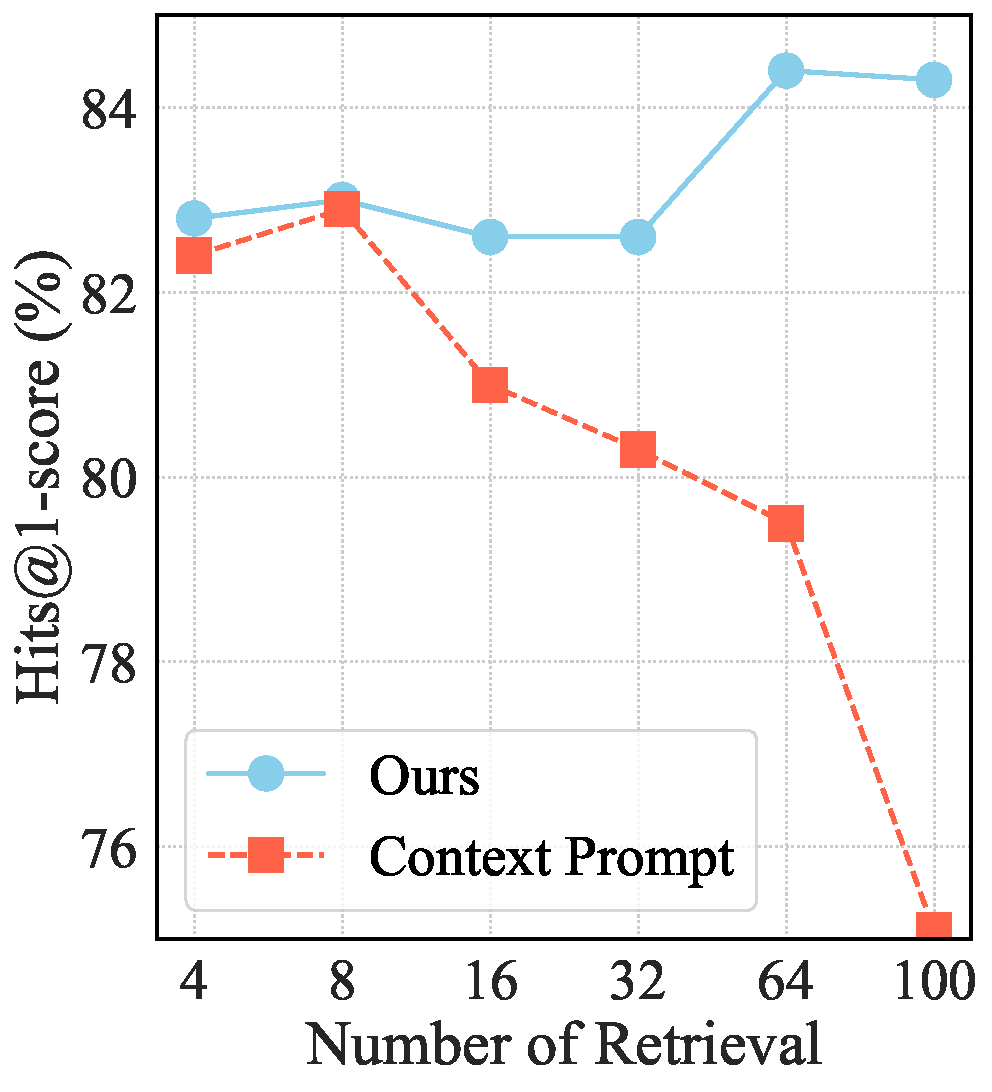
\includegraphics[width=\textwidth]{img/hyperparamter.pdf}
    \caption{Performance vary with the number of Retrieval.}
    \label{fig:topk}
\end{minipage}
\begin{minipage}[c]{0.225\textwidth}
    \centering
    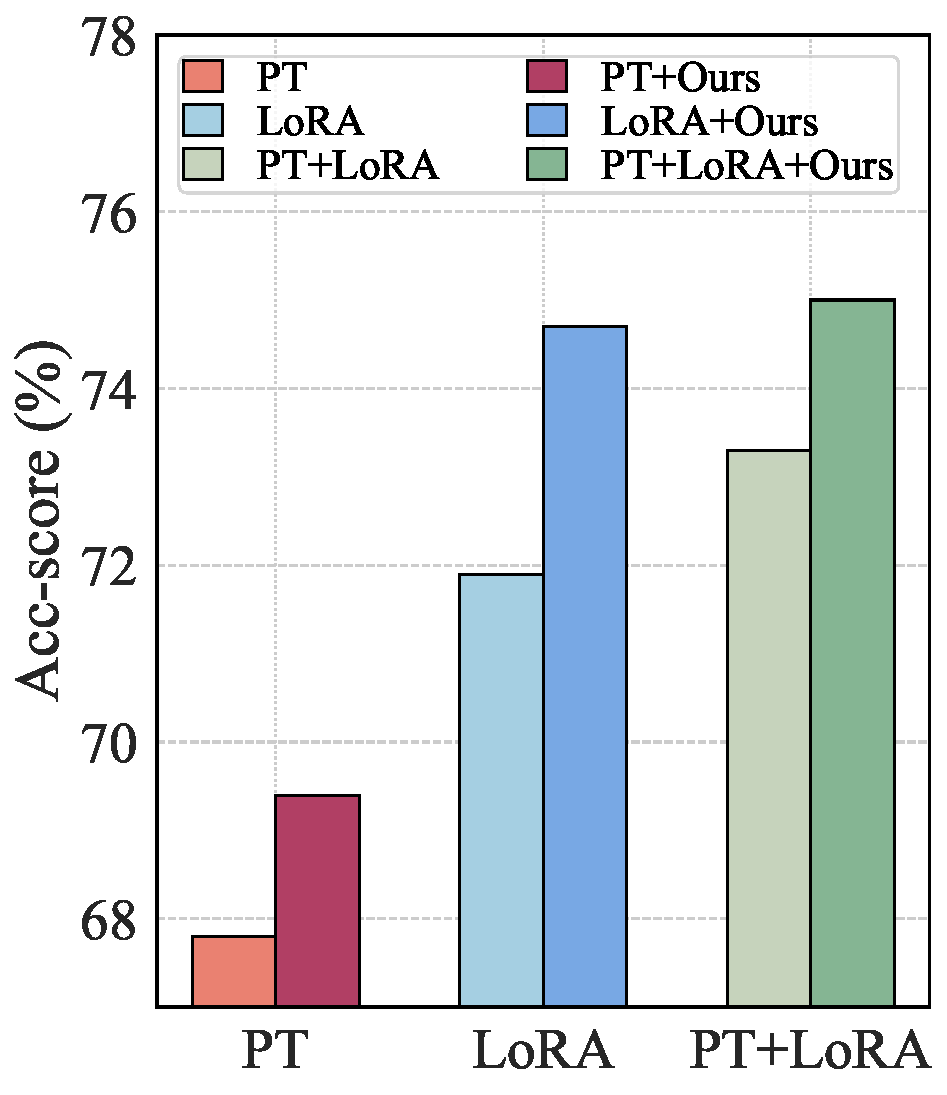
\includegraphics[width=\textwidth]{img/bar.pdf}
    \caption{Combine with different fine-tuning methods.}
    \label{fig:Tuning}
\end{minipage} 
\end{figure}

\begin{table*}[t]
% \setlength\tabcolsep{3pt}  %可以控制列间距
% \renewcommand{\arraystretch}{0.8} %可以控制行间距
\centering
\footnotesize
\begin{tabular}{p{2.7cm}p{14cm}}
\toprule
Question & \textit{what highschool did harper lee go to?} \\
\midrule 
Entity Retrieval & \textit{\ding{172} Harper Lee {[0.9272]}, \ding{173} Senior secondary education {[0.5441]}, 
 \ding{174} Lee Remick {[0.6482]}, \ding{175} Secondary education {[0.5412]}, \ding{176} Barbara Kingsolver {[0.4320]}, \ding{177} High school movement {[0.6758]}}  \\
 \midrule 
Relation Retrieval &  \textit{\ding{172}  people.person.education {[0.9844]},  \ding{173} education.education.institution {[0.9844]},  \ding{174} education.educational\_institution.school\_type {[0.7281]}, \ding{175} education.school.lowest\_grade\_taught {[0.5469]},  \ding{176} education.school\_mascot.school {[0.5431]}, \ding{177} common.topic.notable\_types {[0.8252]}} \\
\midrule 
 Logical Form by \model & \textit{(AND (JOIN common.topic.notable\_types High school) (JOIN (R education.education.institution) (JOIN (R people.person.education) Harper Lee)))} { \CheckmarkBold} \\
\midrule 
 Logical Form by Context Prompt  & \textit{(AND (JOIN \underline{education.educational.institution.school\_type} \underline{School}) (JOIN (R education.education.institution) ( JOIN (R people.person.education) Harper Lee)))} { \XSolidBrush} \\
\bottomrule 
\end{tabular}
\caption{A case study on WebQSP, where the `\textit{[float]}' represents the scores assigned to each retrieval information, indicating the level of influence it has on the model and the \underline{text with underline} means erroneous generation.
}
\label{tab:case}
\end{table*}

\subsection{Efficiency of Fine-Tuning}

In this section, we analyze the efficiency of our method combined with different fine-tuning methods, including Prompt Tuning (PT)~\cite{lester2021prompttuning} and Low-Rank Adaptation (LoRA). To ensure fairness, we conduct fine-tuning experiments without our module by concatenating the retrieved knowledge text with the input context. As shown in Figure \ref{fig:Tuning}, we observe a significant improvement in performance after incorporating \textsc{Amar}, Regardless of whether PT or LoRA is used, our method consistently outperforms baselines.  Notably, the combination of our method with PT+LoRA fine-tuning yields the best results. This highlights the capability of \model to effectively learn from retrieved information, while the direct concatenation of context introduces considerable noise.
Furthermore, we find that LoRA fine-tuning outperforms PT fine-tuning. This can be attributed to the inherent complexity of logical form generation in the KGQA task.  
LoRA has more tunable parameters and can act on all project layers, thus enabling LLMs to better adapt to tasks.


\subsection{Case Study}


In this section, we present a case study to illustrate how our model adaptively learns the importance of retrieval knowledge. We have not presented a case for subgraph retrieval due to its extensive length. As shown in Table \ref{tab:case}, our method is proven effective in assigning high scores to correct entities and relations for entity retrieval and relation retrieval, while irrelevant or misleading information receives low scores. For instance, the entity `\textit{Harper Lee}' received a score of [0.9272], and relation `\textit{people.person.education}' received a score of [0.9844].
Nevertheless, when retrieved text is directly used as the context prompt, it is susceptible to interference from erroneous information in retrieved data. This can result in generating incorrect relations, such as `\textit{education.educational.institution.school type}'. This example highlights that our method not only enhances the performance of LLM in KGQA but also improves the quality of retrieved information by setting weight.

        

\subsection{Analysis of LLM Backbones}
In this section, we investigate the question: \textbf{Does the performance improvement of our method solely come from LLMs?} To answer this, we conduct experiments and compare results using different LLMs as backbones: LLaMA2-7B with fine-tuning, LLaMA2-13B with fine-tuning, and GPT-4 (frozen).
% We observe that when using both LLama2-7b and 13b as backbones, \model outperforms baselines using the same backbone, even better than ToG-R~\cite{TOG} using GPT-4.
In Table \ref{tab:llms}, we observe that \model with LLaMA2-7B and 13B as backbones outperform the baselines using the same backbone, such as ChatKBQA~\cite{chatkbqa}, and both even surpass ToG-R~\cite{TOG} using GPT-4 as the backbone on two datasets.
% Moreover, experiments with LLaMA2-7B even reach slightly better results than with LlaMA2-13B on WebQSP because of over-fitting.
These results suggest that the performance gain of \model is not solely attributed to the use of more capable LLMs but rather to the proposed utilization of the commonality between multi-aspect knowledge and the relevance of the question.
We found that LLaMA2-13B perform worse than LLaMA2-7B on WebQSP. We believe the reason lies in dataset characteristics: the scale of WebQSP (1) is much smaller than that of CWQ, and (2) WebQSP has a maximum complexity, only consisting of 2-hop questions. This may cause the LLaMA2-13B to overfit, leading to reduced performance.


\begin{table}[t]
% \setlength\tabcolsep{3pt}  %可以控制列间距
% \renewcommand{\arraystretch}{1.1} %可以控制行间距
\fontsize{9}{11}\selectfont
\centering
\setlength{\tabcolsep}{3.7mm}{
\begin{tabular}{l|cccc}
\toprule
 \multicolumn{1}{l|}{\multirow{2}{*} {Model}}   & \multicolumn{2}{c}{WebQSP}  & \multicolumn{2}{c}{CWQ}     \\
\cline{2-5}
 \multicolumn{1}{c|}{}   &Acc &Hits@1 &Acc&Hits@1 \\ 
  \hline
  \multicolumn{5}{c}{\textit{GPT-4}} \\
\hline
 ToG-R &- &82.6 &-  & 69.5\\
\hline
\multicolumn{5}{c}{\textit{LLaMA2-7B}} \\
\hline
G-Retriever & - & 70.1& - & - \\
GNN-RAG  &-  & 82.8& -& 62.8\\
ChatKBQA & 73.8 & 83.2 & 73.0 & 82.3 \\
\rowcolor{gray!10}  \model & \textbf{75.2} &\textbf{84.3} & 73.4 & 82.9 \\
 \hline
 \multicolumn{5}{c}{\textit{LLaMA2-13B}} \\
\hline
ChatKBQA & 73.1 & 82.7 & 73.3 & 82.7 \\
\rowcolor{gray!10}  \model & 74.7  &83.3 &\textbf{ 74.5} & \textbf{83.1}\\
\bottomrule
\end{tabular}}
 \caption{Analysis on different LLM backbones. }
\label{tab:llms}
\end{table}



% Answer : Monroe County High School




 